\begin{figure}[h]  
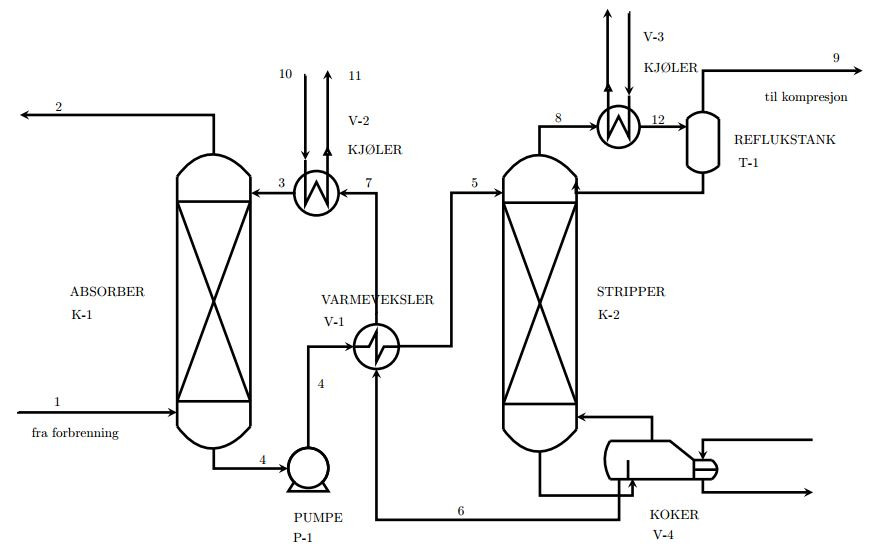
\includegraphics[scale=0.8]{Tegning.JPG}
\centering
\caption{Flytskjema av post-combustion CO\textsubscript{2}-fangst}
\end{figure}

Røyk inn, CO\textsubscript{2} blir løst og absorbert av mea. Som går videre i strøm 4 og blir så pumpet gjennom en varmeveksler som varmer opp løsningen. Så inn i stripper hvor CO\textsubscript{2} går ut av binding med MEA, for så å fordampe ut av løsningen. Mea går gjennom kokeren for å sørge for at mer CO\textsubscript{2} blir frigitt. strøm 6 vil mea gå tilbake gjennom varmeveksleren, så gjennom kjøler for å senke temperaturen. Dermed gjennom strøm 3 tilbake inn i absorberern. I strøm 2 går inertgassene ut + den delen av CO\textsubscript{2} som ikke blir absorbert. 
I reflukstanken vil H\textsubscript{2O} og CO\textsubscript{2} gå utfra stripper gjennom kjøler for å kondensere vanndamp for å skille CO\textsubscript{2} og H\textsubscript{2}O etter å ha blitt kjølt ned i kjøleren. 
Strøm 9 har ren CO\textsubscript{2} mens vannet går tilbake til stripperen. 


Absoerbern så vil CO\textsubscript{2} bli løst i mea løsningen så vil deretter CO\textsubscript{2} bli absorbert/reagere med mea og danne disse to stoffene. Kan vise til rxligning 1+2. Ved lavere temperatur blir mer CO\textsubscript{2} absorbert i mea løsningen og ligge løst i vannet.

I stripperen vil MEA-løsningen varmes opp for å frigji mest mulig CO\textsubscript{2}. Reaksjonene som skjedde i absorben vil bli reversert. Løsningen vil bli varmet opp både for å frigi absorbert CO\textsubscript{2} og for å frigi CO\textsubscript{2} som er løst i vesken. 

Pumpen vil pumpe løsningen gjennom systemet. Vermeveksleren vil vermeveklse strøm 6 mot strøm 4 for å kjøle ned MEA løsningen som skal inn i absorben og for å  varme opp MEA-løsningen som skal inn i stripperen. Disse to strømmene kjøres gjennom varmeveksleren for å energieffektivisere systemet. I kokeren vil MEA-Løsningen bli varmet opp yterligere for å frigi CO\textsubscript{2}-en. Kjølerene vil kjøle ned strømene. i Kljøler 1 vil MEA-løsningen kjøler ned ytterligere før den går inn i absroben, for å lettere kunne absobere CO\textsubscript{2}. I kjøler 2 vil CO\textsubscript{2} og vandamp kjøles ned for å kunne splitte CO\textsubscript{2} og vann i Reflukstanken. I Reflukstanken vil CO\textsubscript{2} og vann bli splittet. 

De to viktigste faktorene i prossessen CO\textsubscript{2}-fangst er absorbantes evne til å absorbere CO\textsubscript{2}(alpha) og hvor raskt aborbanten absorberer CO\textsubscript{2}. De prossesmessige utfordringene 